\documentclass[../main.tex]{subfiles}
\begin{document}
\mainchapter{位相}
\nocite{uchida}
\nocite{introduction-to-topology}

\section{距離空間}
\begin{thmbox}
\begin{definition}
\(\tuple{X, d_{X}}\), \(\tuple{Y, d_{Y}}\)を距離空間とする.
写像\(f\colon X \to Y\)が\keyword{点}\(x \in X\)\keyword{において連続}(continuous at \(x\))であるとは,
任意の\(\varepsilon > 0\)に対して,ある\(\delta > 0\)が存在して,
任意の\(x' \in X\)に対して,\(d_{X}(x', x) < \delta\)ならば\(d_{Y}(f(x'), f(x)) < \varepsilon\)となることをいう.
\definitionlabel{dist-continuity}
\end{definition}
\end{thmbox}


\section{位相空間}
\begin{thmbox}
\begin{definition}
\(X\)を集合とし,\(\symcal{O}\)を\(X\)の部分集合族とする.
\(\symcal{O}\)が以下の\ref{topology-empty}--\ref{topology-union}をみたすとき,
\(\symcal{O}\)の\keyword{位相}(topology)という.
\begin{conditions}
    \item\label{topology-empty} \(\emptyset \in \symcal{O}\)かつ\(X \in \symcal{O}\).
    \item\label{topology-intersection} \(O_1, O_2 \in \symcal{O}\)ならば\(O_1 \cap O_2 \in \symcal{O}\).
    \item\label{topology-union} 集合族\({(O_\lambda)}_{\lambda \in \Lambda}\)が各\(\lambda \in \Lambda\)について\(O_\lambda \in \symcal{O}\)をみたすならば
        \begin{align}
            \bigcup_{\lambda \in \Lambda} \in \symcal{O}.
        \end{align}
\end{conditions}
集合\(X\)とその位相\(\symcal{O}\)の組\((X, \symcal{O})\)を\keyword{位相空間}(topological space)という.\definitionlabel{topology}
\end{definition}
\end{thmbox}

\begin{thmbox}
\begin{definition}
\(\symbb{R}^n\)において
\end{definition}
\end{thmbox}

\(X\)を集合とし,\(\symcal{O}_1\)と\(\symcal{O}_2\)をそれぞれ\(X\)の位相とする.
\(\symcal{O}_1 \subseteq \symcal{O}_2\)が成り立つとき,
\(\symcal{O}_1\)は\(\symcal{O}_2\)より\keyword{粗い}(coarser)\index{粗い@あらい},
または\(\symcal{O}_2\)は\(\symcal{O}_1\)より\keyword{細かい}(finer)\index{細かい@こまかい}という.
\(X\)の位相全体の集合は関係\(\subseteq\)を順序とみなすことにより,半順序集合となる.

任意の集合\(X\)について,最も粗い(coarsest)位相は密着位相であり,最も細かい(finest)位相は離散位相である.
簡単な例として異なる2点からなる集合\(X = \{a, b\}\)を考える.
密着位相\(\{\emptyset, X\}\)に,任意の1点だけからなる集合を1つだけ含めた集合,
すなわち\(\{\emptyset, \{a\}, X\}\)と\(\{\emptyset, \{b\}, X\}\)もまた位相である.
これらを\keyword{Sierpiński\footnote{\pronunciation{Sierpiński}{pl}{ɕɛr{\primarystress}pi\~{\j}sk\textsuperscript{j}i}{シェルピンスキー}}位相}(Sierpiński topology)と呼ぶ.
密着位相\(\{0, X\}\),任意のSierpiński位相\(\symcal{S}\),離散位相\(\wp(X) = \{\emptyset, \{a\}, \{b\}, X\}\)について,\(\{\emptyset, X\} \preceq \symcal{S} \preceq \wp(X)\)が成り立つ.これらを象徴的に図示すると\figref{sierpinski}のようになる.
2つの異なるSierpiński位相は比較可能でないことから,位相の細かさは一般的には全順序にならないことがわかる.

\begin{figure}
    \centering
    \vspace{5.2mm}
    \begin{tikzpicture}
        \draw[thick] (0, 0) ellipse (1.2 and 0.6);
        \node[circle, draw=black, fill=black, inner sep=0pt, outer sep=1pt, minimum size=3pt] at (-0.5, 0) {};
        \node[circle, draw=black, fill=black, inner sep=0pt, outer sep=1pt, minimum size=3pt] at (0.5, 0) {};
        \node at (0, -1.3) {密着位相};

        \draw[thick] (4, 0) ellipse (1.2 and 0.6);
        \node[circle, draw=black, fill=black, inner sep=0pt, outer sep=1pt, minimum size=3pt] at (3.5, 0) {};
        \node[circle, draw=black, fill=black, inner sep=0pt, outer sep=1pt, minimum size=3pt] at (4.5, 0) {};
        \draw[thick] (3.5, 0) circle (0.3);
        \node at (4, -1.3) {Sierpiński位相};

        \draw[thick] (8, 0) ellipse (1.2 and 0.6);
        \node[circle, draw=black, fill=black, inner sep=0pt, outer sep=1pt, minimum size=3pt] at (7.5, 0) {};
        \node[circle, draw=black, fill=black, inner sep=0pt, outer sep=1pt, minimum size=3pt] at (8.5, 0) {};
        \draw[thick] (7.5, 0) circle (0.3);
        \draw[thick] (8.5, 0) circle (0.3);
        \node at (8, -1.3) {離散位相};
    \end{tikzpicture}
    \vspace{4mm}
    \caption{各位相を象徴的に表した図.図における点は集合の元,点を囲む円はその元を含む開集合に対応している.}
    \figlabel{sierpinski}
\end{figure}

\begin{thmbox}
\begin{definition}
\((X, \symcal{O})\)を位相空間とする.\(\symcal{O}\)の部分集合\(\symcal{B}\)について,
任意の\(O \in \symcal{O}\)に対して,ある\(\symcal{B}_0 \subseteq \symcal{B}\)が存在して,
\begin{align*}
    O = \bigcup \symcal{B}_0
\end{align*}
とできるとき,
\(\symcal{B}\)を\(\symcal{O}\)の\keyword{開基}(basis)という.
\end{definition}
\end{thmbox}

\begin{example} \(\symbb{R}\)において開区間全体の集合\(\symcal{I} = \{ (a, b) \mid a,  b \in \symbb{R}\}\)は開基である.
\end{example}

% Singh 1.4.5
\begin{thmbox}
\begin{theorem}
\(X\)を集合とする.部分集合族\(\symcal{B} \subseteq \wp(X)\)が
以下をみたすとき,
\begin{conditions}
    \item \(X = \bigcup \symcal{B}\).
    \item 任意の\(B_1, B_2 \in \symcal{B}\)と\(x \in B_1 \cap B_2\)に対して,
        ある\(B_3 \in \symcal{B}\)が存在して,\(B_1 \cap B_2\)
\end{conditions}
\end{theorem}
\end{thmbox}

\begin{thmbox}
\begin{definition}
\(\tuple{X, \symcal{O}}\)を位相空間とする.
\(\symcal{O}\)の部分集合\(\symcal{S}\)について,
任意の\(O \in \symcal{O}\)と\(x \in O\)に対して,
有限個の\(V_1, \ldots, V_r \)をとって
\(x \in V_1 \cap \cdots \cap V_r\)かつ\(V_1 \cap \cdots \cap V_r \subseteq O\)とできるとき,
\(\symcal{S}\)を\(\symcal{O}\)の\keyword{準開基}(subbasis)という.
\end{definition}
\end{thmbox}

\begin{example} \(\symbb{R}\)において
\begin{align*}
    \symcal{I} =
        \{ (-\infty, x) \mid x \in \symbb{R} \}
        \cup
        \{ (x, \infty) \mid x \in \symbb{R} \}
\end{align*}
は準開基である.\(\symbb{R}\)の開集合を
\end{example}

\section{直積集合と位相}
位相空間\(\tuple{X, \symcal{O}_X}\)と \(\tuple{Y, \symcal{O}_Y}\)が与えられたとき,
直積\(X \times Y\)に位相を定める方法はいくつかある.
その1つは
\begin{align*}
    \symcal{R} = \{ U \times V \mid U \in \symcal{O}_X, V \in \symcal{O}_Y\}
\end{align*}
が生成する位相\(\Box := \Generatedtopology{\symcal{R}}\)を\(X \times Y\)の位相とする方法である.
\(\symcal{R}\)自身は一般的には位相にならない.
例えば\(X = Y = \symbb{R}\)において,
\(X\)の開区間\(U_1, U_2\)と
\(Y\)の開区間\(V_1, V_2\)を
\figref{box-topology}のような位置関係になるようにとる.
このとき\(U_1 \times V_1\)と\(U_2 \times V_2\)は\(\symcal{R}\)の元であるが,
その和集合\((U_1 \times V_1) \cup (U_2 \times V_2)\)は\(\symcal{R}\)の元ではない.

\begin{figure}
    \centering
    \begin{tikzpicture}
        \begin{axis}[
            axis lines=middle,
            axis line style=thick,
            xlabel={$x$},
            ylabel={$y$},
            xtick=\empty,
            ytick=\empty,
            xmin=-0.5,
            xmax=5,
            ymin=-0.5,
            ymax=3,
            samples=200,
            clip=false
        ]
        % vertical lines
        \addplot[dotted, sBlue] coordinates {(0.5, -0.25) (0.5, 2.5)};
        \addplot[dotted, sRed] coordinates {(1.5, -0.25) (1.5, 2.5)};
        \addplot[dotted, sBlue] coordinates {(2, -0.25) (2, 3)};
        \addplot[dotted, sRed] coordinates {(3, -0.25) (3, 3)};
        \addplot[ultra thick, sBlue] coordinates {(0.03, 0.5) (0.03, 1.5)};
        \addplot[ultra thick, sRed] coordinates {(-0.03, 1) (-0.03, 2)};
        % horizontal lines
        \addplot[dotted, sBlue] coordinates {(-0.25, 0.5) (3.5, 0.5)};
        \addplot[dotted, sRed] coordinates {(-0.25, 1) (3.5, 1)};
        \addplot[dotted, sBlue] coordinates {(-0.25, 1.5) (3.5, 1.5)};
        \addplot[dotted, sRed] coordinates {(-0.25, 2) (3.5, 2)};
        \addplot[ultra thick, sBlue] coordinates {(0.5, 0.03) (2, 0.03)};
        \addplot[ultra thick, sRed] coordinates {(1.5, -0.03) (3, -0.03)};

        \node at (axis cs:-0.2, -0.2) {$O$};
        \node at (axis cs:1.25, -0.2) {\textcolor{sBlue}{$U_1$}};
        \node at (axis cs:2.25, -0.2) {\textcolor{sRed}{$U_2$}};
        \node at (axis cs:0.3, 1) {\textcolor{sBlue}{$V_1$}};
        \node at (axis cs:-0.2, 1.5) {\textcolor{sRed}{$V_2$}};
        \node at (axis cs:0.8, 1.7) {\textcolor{sBlue}{$U_1 \times V_1$}};
        \node at (axis cs:2.25, 2.2) {\textcolor{sRed}{$U_2 \times V_2$}};
        \node[anchor=west] at (axis cs:3.2, 1.25) {$(U_1 \times V_1) \cup (U_2 \times V_2)$};

        \fill[pattern=north east lines, pattern color=sBlue] (axis cs:0.5, 1.5) rectangle (axis cs:2, 0.5);
        \fill[pattern=north west lines, pattern color=sRed] (axis cs:1.5, 2) rectangle (axis cs:3, 1);

        \addplot[thick] coordinates {%
            (0.5, 1.5)
            (0.5, 0.5)
            (2, 0.5)
            (2, 1)
            (3, 1)
            (3, 2)
            (1.5, 2)
            (1.5, 1.5)
        } -- cycle;

        \end{axis}
    \end{tikzpicture}
    \caption{\(\symbb{R} \times \symbb{R}\)の箱位相の元の例.}\figlabel{box-topology}
\end{figure}

一般に位相空間の族\(({(X_\lambda, \symcal{O}_\lambda))}_{\lambda \in \Lambda}\)が与えられたとき,
\begin{align*}
    \symcal{R} = \left\{
        \prod_{\lambda \in \Lambda} O_\lambda
        \relmiddle{|}
        \text{任意の\(\lambda \in \Lambda\)について\(O_\lambda \in \symcal{O}_\lambda\)}
        \right\}
\end{align*}
が生成する位相\(\Box := \Generatedtopology{\symcal{R}}\)を\({((X_\lambda, \symcal{O}_\lambda))}_{\lambda \in \Lambda}\)の\keyword{箱位相}(box topology)という.

\begin{thmbox}
\begin{proposition}
\(\symbb{R} \times \symbb{R}\)の箱位相\(\Box\)は\(\symbb{R}^2\)の通常の位相\(\symcal{O}\)と一致する.
\end{proposition}
\end{thmbox}

\begin{proof} (\(\Box \subseteq \symcal{O}\))任意の\(O \in \Box\)をとる.
\end{proof}

\begin{thmbox}
\begin{definition}
位相空間\(\tuple{X, \symcal{O}}\)の部分集合\(A\)が\(\overline{A} = X\)をみたすとき,
\(A\)は\(X\)において\keyword{稠密}(dense)であるという.
\end{definition}
\end{thmbox}

稠密であることは次のように言い換えられる.

\begin{thmbox}
\begin{proposition}
位相空間\(\tuple{X, \symcal{O}}\)の部分集合\(A\)が稠密であることは,
任意の\(O \in \symcal{O} \setminus \{\emptyset\}\)について\(A \cap O \neq \emptyset\)が成り立つことと同値である.
\propositionlabel{dense-paraphrase}
\end{proposition}
\end{thmbox}

\begin{proof}(\(\Rightarrow\))任意の\(O \in \symcal{O} \setminus \{\emptyset\}\)をとる.
\(O\)は空でないから,ある\(x \in O\)が存在する.
\(x \in O \subset X\)であり,仮定\(X \subseteq \overline{A}\)より\(x \in \overline{A}\)である.
したがって触点の性質から\(A \cap O \neq \emptyset\)が成り立つ.

\noindent (\(\Leftarrow\))任意の\(x \in X\)をとる.
仮定から\(x\)の任意の開近傍\(V\)について\(A \cap V \neq \emptyset\)が成り立つ.
したがって\(x \in \overline{A}\),すなわち\(X \subseteq \overline{A}\)が示された.
\end{proof}

\begin{thmbox}
\begin{definition}
\({\tuple{\tuple{X_\lambda, \symcal{O}_\lambda}}}_{\lambda \in \Lambda}\)を位相空間の族とし,
\(X = \prod_{\lambda \in \Lambda} X_\lambda\)とする.
\(\Lambda\)の任意の有限部分集合全体の集合を\(\symcal{I}\)とする.任意の\(I \in \symcal{I}\)について
\begin{align*}
    \Pi_I = \left\{ f\colon \Lambda \to \bigcup_{\lambda \in \Lambda} X_\lambda \relmiddle{|} \text{\parbox{7cm}{\(f(i) \in \symcal{O}_i\) for all \(i \in I\) and \(f(\lambda) \in X_\lambda\) for all \(\lambda \in \Lambda \setminus I\)}}\right\}
    % \Pi_I = \left\{ f\colon \Lambda \to \bigcup_{\lambda \in \Lambda} X_\lambda \relmiddle{|} \text{各\(i \in I\)について\(\symcal{O}_i\)かつ\(\lambda \in \Lambda \setminus I\)について\(f(\lambda) \in X_\lambda\)}\right\}
\end{align*}
と定義する.このとき\(\bigcup_{I \in \symcal{I}} \Pi_I\)が生成する位相\(\symcal{O}:=\tau[\bigcup_{I \in \symcal{I}}\Pi_I]\)を\(X\)の\keyword{直積位相}(product topology)という.
\end{definition}
\end{thmbox}

直積\(X = \prod_{\lambda \in \Lambda} X_\lambda\)について,その位相としては特に断らない限り上で定義した\(\symcal{O}\)をとる.組\(\tuple{X, O}\)を\({\tuple{\tuple{X_\lambda, \symcal{O}_\lambda}}}_{\lambda \in \Lambda}\)の\keyword{直積位相空間}(product topological space)と呼ぶ.


\begin{thmbox}
\begin{theorem}[(Tikhonovの定理)]
\({\tuple{\tuple{X_\lambda, \symcal{O}_\lambda}}}_{\lambda \in \Lambda}\)を位相空間の族とする.
各\(\lambda \in \Lambda\)で\(X_\lambda\)がコンパクトならば,
\({\tuple{\tuple{X_\lambda, \symcal{O}_\lambda}}}_{\lambda \in \Lambda}\)の直積位相空間もまたコンパクトである.
\end{theorem}
\end{thmbox}

\section{連続写像}
\begin{thmbox}
\begin{definition}
\(\tuple{X, \symcal{O}_{X}}\), \(\tuple{Y, \symcal{O}_{Y}}\)を位相空間とする.
写像\(f\colon X \to Y\)が点\(x \in X\)において連続であるとは,
\(f(x)\)の\(\tuple{Y, \symcal{O}_{Y}}\)における任意の近傍\(V\)に対して,
\(\tuple{X, \symcal{O}_{X}}\)における\(x\)のある近傍\(U\)が存在して,\(f(U) \subseteq V\)となることをいう.
\definitionlabel{topology-continuity}
\end{definition}
\end{thmbox}


\section{ネット}
\begin{thmbox}
\begin{definition}
空でない集合\(A\)上と,以下の\ref{directed-set-reflex}--\ref{directed-set-upper}を満たす
関係\(\preceq\)の組\(\tuple{A, \preceq}\)を\keyword{有向集合}(directed set)という.
関係\(\preceq\)が明らかな場合は\(\tuple{A, \preceq}\)を単に\(A\)と書く.
\begin{conditions}
    \item\label{directed-set-reflex} (反射律)任意の\(\alpha \in A\)について\(\alpha \preceq \alpha\).
    \item\label{directed-set-trans} (推移律)任意の\(\alpha, \beta, \gamma \in A\)について\(\alpha \preceq \beta\)かつ\(\beta \preceq \gamma\)ならば\(\alpha \preceq \gamma\).
    \item\label{directed-set-upper} 任意の\(\alpha, \beta \in A\)に対して\(\alpha \preceq \gamma\)かつ\(\beta \preceq \gamma\)をみたす\(\gamma \in A\)が存在する.
\end{conditions}
\end{definition}
\end{thmbox}

上の定義の\ref{directed-set-reflex}と\ref{directed-set-trans}は順序の公理から反対称律を除いたものである.
この\(2\)つを満たす関係を\keyword{前順序}(preorder)と呼ぶ\footnote{%
前順序を「ぜんじゅんじょ」と読んでしまうと全順序と紛らわしいので「まえじゅんじょ」と読んだり,
preorderと呼んだりするほうがいいだろう.}.有向集合に用いて列の一般化であるネットが定義される.
\ref{directed-set-upper}は数列のように無限に続くこと、また以下の図のようにずっと分岐していくことがないことを要請している.

\begin{figure}
    \centering
    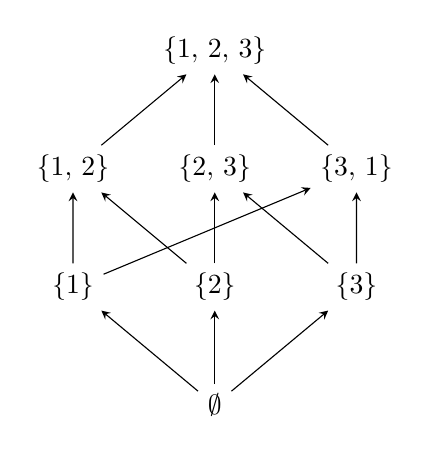
\begin{tikzpicture}[scale=.6]
      \node (emptyset) at (0, -2.5) {$\emptyset$};
      \node (p1) at (-3, 0) {$\{1\}$};
      \node (p2) at (0, 0) {$\{2\}$};
      \node (p3) at (3, 0) {$\{3\}$};
      \node (p12) at (-3, 2.5) {$\{1,\,2\}$};
      \node (p23) at (0, 2.5) {$\{2,\,3\}$};
      \node (p31) at (3, 2.5) {$\{3,\,1\}$};
      \node (p123) at (0, 5) {$\{1,\,2,\,3\}$};
      \draw[-stealth,] (emptyset) -- (p1);
      \draw[-stealth,] (emptyset) -- (p2);
      \draw[-stealth,] (emptyset) -- (p3);
      \draw[-stealth,] (p1) -- (p12);
      \draw[-stealth,] (p1) -- (p31);
      \draw[-stealth,] (p2) -- (p12);
      \draw[-stealth,] (p2) -- (p23);
      \draw[-stealth,] (p3) -- (p23);
      \draw[-stealth,] (p3) -- (p31);
      \draw[-stealth,] (p12) -- (p123);
      \draw[-stealth,] (p23) -- (p123);
      \draw[-stealth,] (p31) -- (p123);
    \end{tikzpicture}
    \caption{TODO}
    \figlabel{subset-order-hasse-diagram}
\end{figure}

\begin{thmbox}
\begin{definition}
有向集合\(\Lambda\)から集合\(X\)への写像\(f \colon \Lambda \to X\)を\(X\)の\keyword{ネット}(net in \(X\))という.
\end{definition}
\end{thmbox}

ネットはしばしば列や族と同様に\(\Family{x}\)や単に\(\SimpleFamily{x}\)のように書かれる.
以降,厳密に使い分けることはせず,\(f, g\)のような表記と\(\Family{x}\)のような表記を併せて用いる.

\begin{exa}
Riemann\footnote{\pronunciation{Riemann}{de}{ˈʀiːman}{リーマン}}積分の定義に用いられる\keyword{分割}(partition)\index{ぶんかつ@分割 partition}は有向集合の例である.
分割とは,区間\(I = [a, b]\)が与えられたとき,\(a = x_0 < x_1 < \cdots < x_n = b\)を満たすような点の集合\(\{x_0, \ldots, x_n\}\)のことをいう.
2つの分割\(\Delta = \{x_0, \ldots, x_n\}\)と\(\Delta' = \{y_0, \ldots, y_m\}\)について\(\Delta \subseteq \Delta' \)が成り立つとき,\(\Delta'\)は\(\Delta\)の\keyword{細分}(refinement)\index{さいぶん@細分 refinement}であるという.
\(\Delta'\)が\(\Delta\)の細分であるとき関係\(\Delta \preceq \Delta'\)が成り立つと定める.このとき\(I\)の分割全体の集合は有向集合である.有向集合の定義\ref{directed-set-reflex}と\ref{directed-set-trans}が成り立つのは明らかである.
\ref{directed-set-upper}については,分割\(\Delta\)と\(\Delta'\)が与えられたとき,\(\Delta \cup \Delta'\)の元を用いた分割\(\Delta^*\)について\(\Delta \preceq \Delta^*\)と\(\Delta' \preceq \Delta^*\)となることからわかる.

閉区間\(I\)上で定義される実数値関数\(f\)について,\(I\)の分割\(\Delta = (x_0, \ldots, x_n)\)による\keyword{過剰和}(upper sum)と\keyword{不足和}(lower sum)を以下で定義する:
\begin{gather}
    U(f, \Delta) := \sum_{i = 1}^n \sup \{ f(x) \mid x \in [x_{i - 1}, x_i] \} (x_i - x_{i - 1}), \\
    L(f, \Delta) := \sum_{i = 1}^n \inf \{ f(x) \mid x \in [x_{i - 1}, x_i] \} (x_i - x_{i - 1}).
\end{gather}
このとき\(\Delta \mapsto U(f, \Delta)\), \(\Delta \mapsto L(f, \Delta)\)はそれぞれネットになっている.
\end{exa}

\pgfmathdeclarefunction{curve}{1}{%
    \pgfmathparse{1.7 * sin(0.72 * deg(#1)) + 2.2}%
}

\begin{figure}
    \centering
    \begin{tikzpicture}
        \pgfdeclarepatternformonly{north east lines wide}
           {\pgfqpoint{-1pt}{-1pt}}
           {\pgfqpoint{10pt}{10pt}}
           {\pgfqpoint{9pt}{9pt}}
           {%
             \pgfsetlinewidth{0.4pt}
             \pgfpathmoveto{\pgfqpoint{0pt}{0pt}}
             \pgfpathlineto{\pgfqpoint{9.1pt}{9.1pt}}
             \pgfusepath{stroke}
           }
        \begin{axis}[
            domain=-0.5:8,
            samples=200,
            axis lines=middle,
            xlabel={\(x\)},
            ylabel={\(y\)},
            xmin=-0.8,
            xmax=8.5,
            ymin=-2.0,
            ymax=5,
            xtick=\empty,
            xticklabels=\empty,
            ytick=\empty,
            yticklabels=\empty,
            width=15cm,
            height=7cm,
        ]
        \node at (axis cs: -0.25, -0.4) {\(O\)};

        \pgfplotsinvokeforeach{0, ..., 4}{%
            \node at (axis cs: {#1 + 1}, -0.1) [anchor=north] {\(x_#1\)};
            \node at (axis cs: {#1 + 1}, -0.6) [anchor=north] {\rotatebox[origin=c]{90}{\(=\)}};
        }
        \pgfplotsinvokeforeach{2, ..., 5}{%
            \node at (axis cs: #1, -1.2) [anchor=north] {\(y_#1\)};
        }

        \node at (axis cs: 1, -1.2) [anchor=north] {\(y_0\)};
        \node at (axis cs: 1.5, -1.2) [anchor=north] {\(y_1\)};

        \node at (axis cs: 5.5, -0.5) [anchor=west] {\(\Delta = \{x_0, \ldots, x_4\}\)};
        \node at (axis cs: 5.5, -1.5) [anchor=west] {\(\Delta' = \{y_0, \ldots, y_5\}\)};

        \addplot[sBlue, thick] {curve(x)};
        \pgfmathsetmacro\dx{1};
        \foreach \ii in {1, ..., 4} {%
            \pgfmathsetmacro\xleft{\ii * \dx};
            \pgfmathsetmacro\xright{\ii * \dx + \dx};
            \pgfmathsetmacro\yleft{curve(\xleft)};
            \pgfmathsetmacro\yright{curve(\xright)};
            \pgfmathsetmacro\yminimum{min(\yleft, \yright)};
            \addplot [
                pattern=north east lines wide,
                pattern color=sRed,
                draw,
            ] coordinates {%
                (\xleft, 0)
                (\xleft, \yminimum)
                (\xright, \yminimum)
                (\xright, 0)
                (\xleft, 0)
            };
        }
        \addplot [
            pattern=north east lines wide,
            pattern color=sRed,
            draw,
        ] coordinates {%
            (1.5, 0)
            (1.5, {curve(1.5)})
            (2, {curve(1.5)})
            (2, 0)
            (1.5, 0)
        };
        \draw[dashed] (axis cs: 1.5, -0) -- (axis cs: 1.5, -1.2);
        \end{axis}
    \end{tikzpicture}
\end{figure}

\begin{thmbox}
\begin{definition}
ネット\(f\colon A \to X\)について,ある\(\alpha \in A\)が存在して,任意の\(\alpha' \geq \alpha\)について
\(f(\alpha') \in Y\)が成り立つとき,\(f\)は\keyword{最終的に}\(Y\)\keyword{に入る}\((f\) is eventually in \(Y)\)という.
\end{definition}
\end{thmbox}

列\(\Sequencen{x}\)の部分列(subsequence)は,狭義単調増加関数\(\varphi\colon\PositiveInteger\to\PositiveInteger\)を用いて\(\Subsequence{x}\)と表されるような列のことである.
あるいは列\(f\)の部分列は合成写像\(f\circ \varphi\)であると言い換えてもよい.
ネットの部分列に対応するものはサブネットと呼ばれ,以下のように定義される:

\begin{thmbox}
\begin{definition}[(サブネット)] \(A\)の部分集合\(B\)
    \begin{conditions}
        \item\label{subnet-comp} \(g = f \circ \varphi\).
        \item\label{subnet-exists-beta} 任意の\(\alpha \in A\)に対して,ある\(\beta \in B\)が存在して,\(\beta' \succeq \beta\)ならば\(\alpha \preceq \varphi(\beta')\)が成り立つ.
    \end{conditions}
\end{definition}
\end{thmbox}

部分列がサブネットであることを確認する.
\ref{subnet-comp}は明らかなので,\ref{subnet-exists-beta}について確認する.
一般に,任意の正整数\(n\)と狭義単調増加\(\varphi\colon\PositiveInteger\to\PositiveInteger\)について\(n \leq \varphi(n)\)が成り立つことを示す.
\(n = 1\)のとき\(\varphi(1) \geq \min \PositiveInteger = 1\)となり成り立つ.
\(n\)まで\(n \leq \varphi(n)\)が成り立っていると仮定し,\(n + 1 \leq \varphi(n + 1)\)が成り立つことを示す.
\(\varphi\)が狭義単調増加であることから\(\varphi(n) < \varphi(n + 1)\)が成り立つ.
また仮定から\(n  \leq \varphi(n)\)なので,\(n \leq \varphi(n) < \varphi(n + 1)\)が成り立つ.
もし\(n < \varphi(n)\)ならば,\(n + 1 \leq \varphi(n) \leq \varphi(n + 1)\)となり成り立つ.
もし\(n = \varphi(n)\)ならば,\(n + 1 = \varphi(n) + 1 < \varphi(n + 1) + 1\)となり成り立つ.
よって任意の\(n \in \PositiveInteger\)で\(n \leq \varphi(n)\)となる.
\ref{subnet-exists-beta}の確認に戻る.
\(\tuple{A, \preceq_A} = \tuple{B, \preceq_B} = \tuple{\PositiveInteger, \leq}\)とする.
\(\alpha = n\)に対して\(\beta = \varphi(n)\)とすれば,
任意の\(\beta' \geq \beta\)について\(\alpha = n \leq \varphi(n) = \beta \leq \beta' \leq \varphi(\beta')\)となる.

\begin{exa}サブネットであるが部分列ではない例として
\end{exa}

\begin{thmbox}
\begin{definition}
\(S\)を\(X\)の任意の部分集合とする.
\(X\)のネット\(f\)が,\(S\)または\(X \setminus S\)のいずれかに最終的に含まれるならば,
\(f\)は\keyword{普遍的な}(universal)ネットであるという.
\end{definition}
\end{thmbox}

\begin{thmbox}
\begin{definition}
\(\tuple{X, \symcal{O}}\)を位相空間とする.
\(x\)の任意の開近傍\(U\)について,ある\(\lambda_0 \in \Lambda\)が存在して,
任意の\(\lambda \preceq \lambda_0\)について\(x_\lambda \in U\)が成り立つとき,
\keyword{\(\SimpleFamily{x}\)は\(x\)に収束する}(\(\SimpleFamily{x}\) converges to \(x\))といい,
\(x_\lambda \to x\)と書く.
この\(x\)を\(\SimpleFamily{x}\)の\keyword{極限}(limit point)という.
\end{definition}
\end{thmbox}

一般の位相空間において,ネットは複数の極限をもつことがある.
たとえば\(X = \{0, 1\}\)に密着位相\(\symcal{O} = \{\emptyset, X\}\)を入れた\(\tuple{X, \symcal{O}}\)を考える.
このとき任意の\(f\colon \PositiveInteger \to \{0, 1\}\)は\(0\)と\(1\)に収束する.

\begin{thmbox}
\begin{definition}
\(X\)を位相空間とする.
\(X\)の任意の異なる\(2\)点\(x, y\)に対し,
\(x\)の近傍\(U\)と\(y\)の近傍\(V\)で\(U \cap V = \emptyset\)をみたすものがとれるとき,
\(X\)を\keyword{Hausdorff{\footnotemark}空間}(Hausdorff space)という.
\end{definition}
\end{thmbox}

\begin{thmbox}
\begin{proposition}
Hausdorff空間においてネットが収束するならば,その極限はただ\(1\)つである.
\end{proposition}
\end{thmbox}

\begin{proof} \(X\)をHausdorff空間とする.
任意の収束するネット\(\Family{x}\)をとり,その極限を\(x\)とする.
また\(\Family{x}\)が\(x\)とは異なる点\(y\)にも収束すると仮定する.
\(X\)がHausdorff空間なので\(x\)の開近傍\(U\)と\(y\)の開近傍\(V\)で\(U \cap V = \emptyset\)であるようなものをとることができる.\(x_\lambda \to x\)より,ある\(\lambda_0 \in \Lambda\)が存在して,
任意の\(\lambda \succeq \lambda_0\)で\(x_\lambda \in U\)が成り立つ.
また\(x_\lambda \to y\)より,ある\(\lambda_0' \in \Lambda\)が存在して,
任意の\(\lambda \succeq \lambda_0\)で\(x_\lambda \in V\)が成り立つ.
したがって\(\lambda \succeq \max \{\lambda_0, \lambda_0'\}\)ならば
\(x_\lambda \in U \cap V\)となるが,これは\(U \cap V = \emptyset\)であったことと矛盾する.
\end{proof}

\footnotetext{\pronunciation{Hausdorff}{de}{ˈha\invbreve{ʊ}sdɔʀf}{ハウスドルフ}}
